\item \textbf{{[}ALVL/9597/2018/P1/Q4{]} }

In a computer game, a player (\textquotedbl\texttt{O}\textquotedbl )
moves around a maze measuring 10 metres by 11 metres to collect a
prize (\textquotedbl\texttt{P}\textquotedbl ). The prize is placed
at a random position within the maze. The prize position is not where
a wall (\textquotedbl\texttt{X}\textquotedbl ) appears in the maze.
An empty position is indicated with a full-stop (\textquotedbl\texttt{.}\textquotedbl ). 

The maze is represented on the screen by a rectangular grid. Each
square metre of the maze is represented by an x-coordinate and a y-coordinate.
The top left square metre of the puzzle display has x = \texttt{0}
and y = \texttt{0}.

The player moves left, right, up or down according to a direction
entered by the user. The game is turn-based; a user enters the direction,
their player moves one position in that direction. lithe direction
would place the player on a well, then the player does not move. The
maze is displayed after each move.
\begin{center}
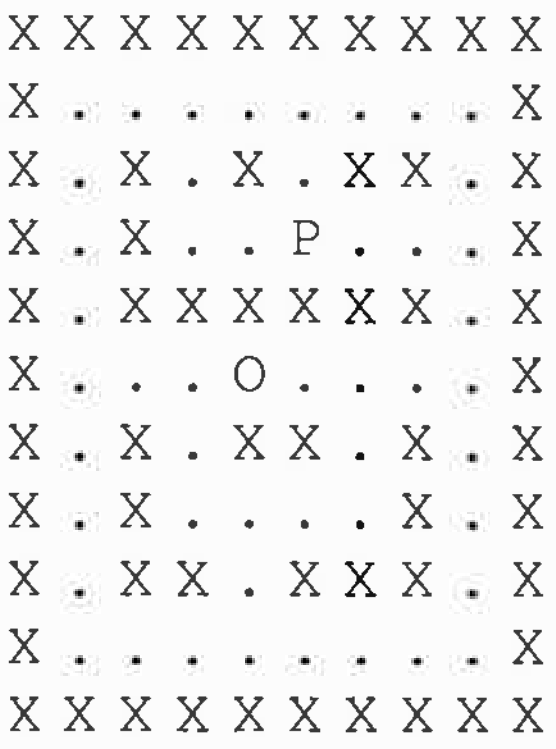
\includegraphics[width=0.25\paperwidth]{C:/Users/Admin/Desktop/Github/question_bank/LyX/static/img/9597-ALVL-2018-P1-Q4}
\par\end{center}

\subsubsection*{Task 4.1}

Write a program to display the maze as shown.
\begin{itemize}
\item The maze should be stored in a suitable data structure.
\item The data structure will allow fixed loop(s) to be used to display
the maze.
\end{itemize}
The maze is given in the text file \texttt{MAZE.TXT}. You may read
in the data from this file or place the data in your program using
any suitable method.

\subsubsection*{Evidence 14}

Your program code. \hfill{} {[}6{]}

\subsubsection*{Task 4.2}

The prize is placed randomly on the maze. It cannot appear in the
same grid position as a wall (\textquotedbl\texttt{X}\textquotedbl ).

Add to your program code to place the prize at a random position.

Take a screenshot of the maze with the prize displayed in it.

\subsubsection*{Evidence 15}

Your program code. \hfill{}{[}4{]}

\subsubsection*{Evidence 16}

A screenshot of the maze as output by your program. \hfill{} {[}1{]}

The player is represented by the character \textquotedbl\texttt{O}\textquotedbl .
The character starts the game in a central position on the grid, for
example, x = \texttt{4} and y = \texttt{5}. 

To move the character, the user is prompted for a direction. The following
are valid inputs:
\begin{center}
\begin{tabular}{|c|l|}
\hline 
\textbf{Input character} & \hspace{0.05\columnwidth}\textbf{Action}\tabularnewline
\hline 
\texttt{``U''} & Player moves up\tabularnewline
\hline 
\texttt{``D''} & Player moves down\tabularnewline
\hline 
\texttt{``L''} & Player moves left\tabularnewline
\hline 
\texttt{``R''} & Player moves right\tabularnewline
\hline 
\texttt{``''} & Continue with previous move.\tabularnewline
 & If no previous move, do nothing\tabularnewline
\hline 
\end{tabular}
\par\end{center}

If the next position for the player (\textquotedbl\texttt{O}\textquotedbl )
is a wall (\textquotedbl\texttt{X}\textquotedbl ), then the player
stays in their current position; this is called collision detection.

When the player enters the move, a new position for the player (\textquotedbl\texttt{O}\textquotedbl )
is calculated and the maze is displayed. The previous position is
changed back to a \textquotedbl .\textquotedbl{} when the player
has a new position. The moves are repeated until the player is at
the same position as the prize.

\subsubsection*{Task 4.3}

Add to your program code to:
\begin{itemize}
\item place the player on the grid at a central position on the grid
\item take in and validate a direction
\item calculate a new position
\item check this position is not a wall
\item update the grid so that the previous position of \textquotedbl\texttt{O}\textquotedbl{}
is replaced with a \textquotedbl{} . \textquotedbl{} and \textquotedbl\texttt{O}\textquotedbl{}
is located in its new position
\item continue this until the player is at the same position as the prize.
\end{itemize}

\subsubsection*{Evidence 17}

Your program code. \hfill{} {[}16{]}

When the player and the prize are at the same position, the message
\textquotedblleft Player has reached the prize\textquotedblright{}
is displayed and the game ends.

\subsubsection*{Task 4.4}

Add to your program, code to end the game when this condition is met,
and display the required message. Produce screenshots to show key
elements of your program are functioning.

The screenshots required are:
\begin{itemize}
\item entering each direction
\item player changing position
\item end of game
\end{itemize}

\subsubsection*{Evidence 18}

Your program code. \hfill{} {[}1{]}

\subsubsection*{Evidence 19}

Screenshots of:
\begin{itemize}
\item entering each direction
\item player changing position
\item end of game (player wins) \hfill{} {[}2{]}
\end{itemize}